\section{Modularity}

The idea of modularity is to partition the overall development effort, support independent testing and analysis of components, decouple parts so they can be modified individually and dividing a large system in mind-sized chunks.


\subsection{Coupling}

Coupling measures interdependence between different modules. A thigh / high coupling means that modules cannot be developed, tested, changed, understood or reused in isolation. Therefore, we want low coupling for correct and maintainable software.

\subsubsection{Data Coupling}

Modules that expose their internal data representation become tightly coupled to their clients (representation exposure). It prevents modules from maintaining strong invariant and concurrency requires complex synchronization. Similarly, data representations often include sub-objects, exposing these can lead to unexpected side effects. \\

One way of preventing this is to restrict the access to data - forcing clients to access the data representation through a narrow interface. Avoid exposure of sub-objects and prevent the leaks of any references to these sub-objects. \\

Modules also get coupled by operating on shared data structures (e.g. compiler working on syntax tree). This can be avoided by making the data structure immutable, however changing the data representation remains a problem and having to copy it can lead to run-time and memory overhead. \\

The flyweight pattern is one example that tries to maximize sharing of immutable objects, it is for example used in Java for constant strings.

\subsubsection{Procedural Coupling}

Modules are coupled to other modules whose methods they call. Callers cannot be reused without the callee modules and changing a signature in the callee requires changing the caller. \\

This can be prevented by moving code and even duplicating functionality to avoid dependency. Another solution could be to change to a event based system. Components may generate events and register for events from other components using a callback. Event generators do not know which components will be affected by their events (loss of control). \\

One common event based architecture is Model-View-Controller. The model contains the core functionality and data, the view is responsible for displaying information and the controller handles user inputs. All communication happens via events, the models and the views are decoupled through the controllers.
\begin{center}
	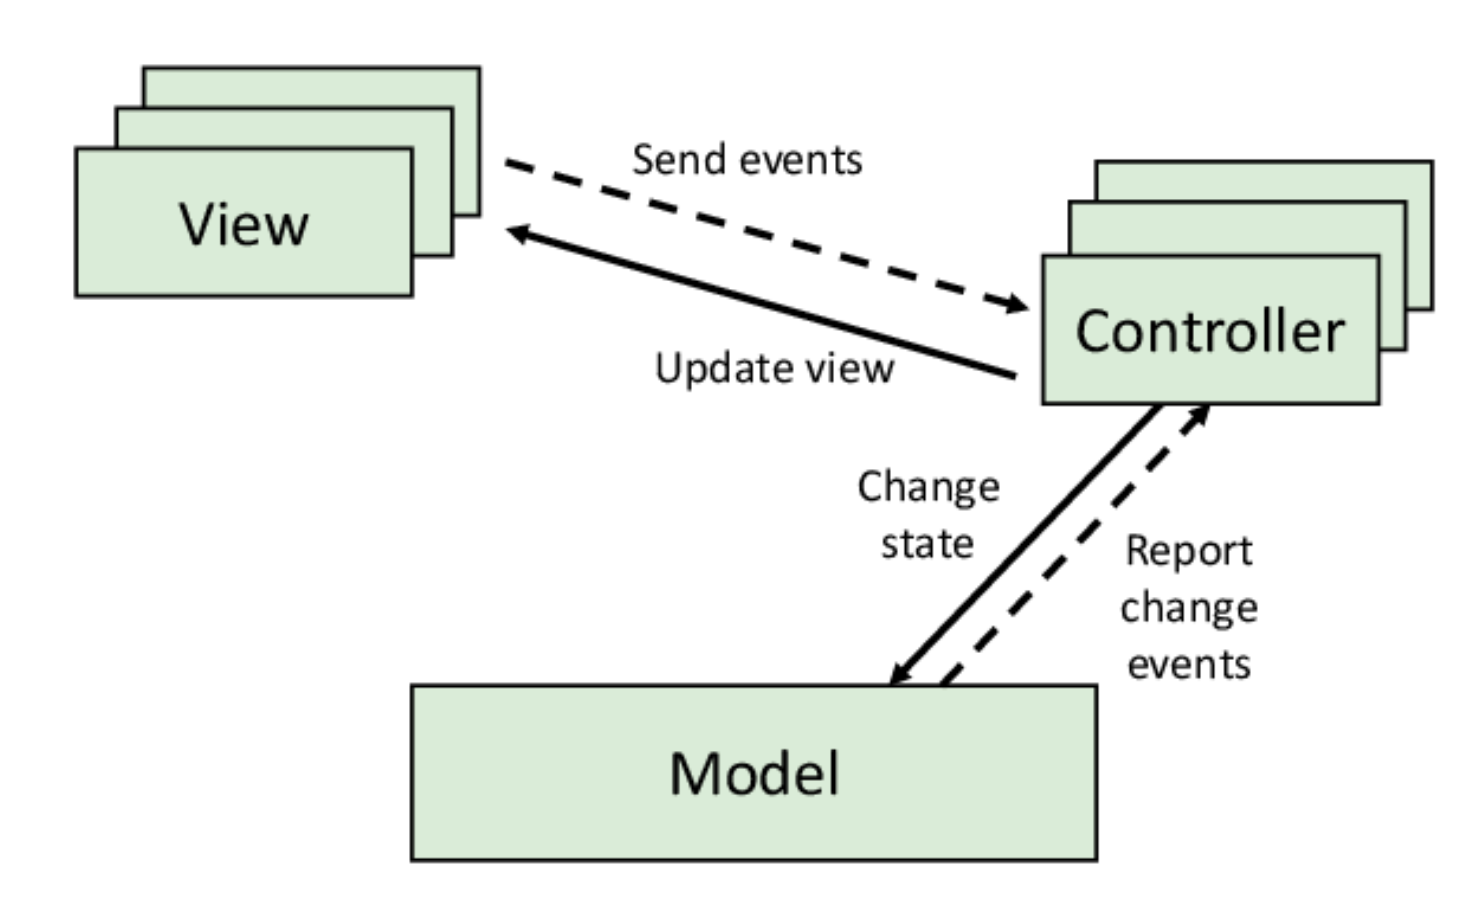
\includegraphics[width=0.7\columnwidth]{assets/mvc}
\end{center}

\subsubsection{Class Coupling}

Inheritance couples the subclass to the superclass, changes in the superclass may break the subclass. To solve this, we can replace (multiple) inheritance by subtyping and delegation.
\begin{center}
	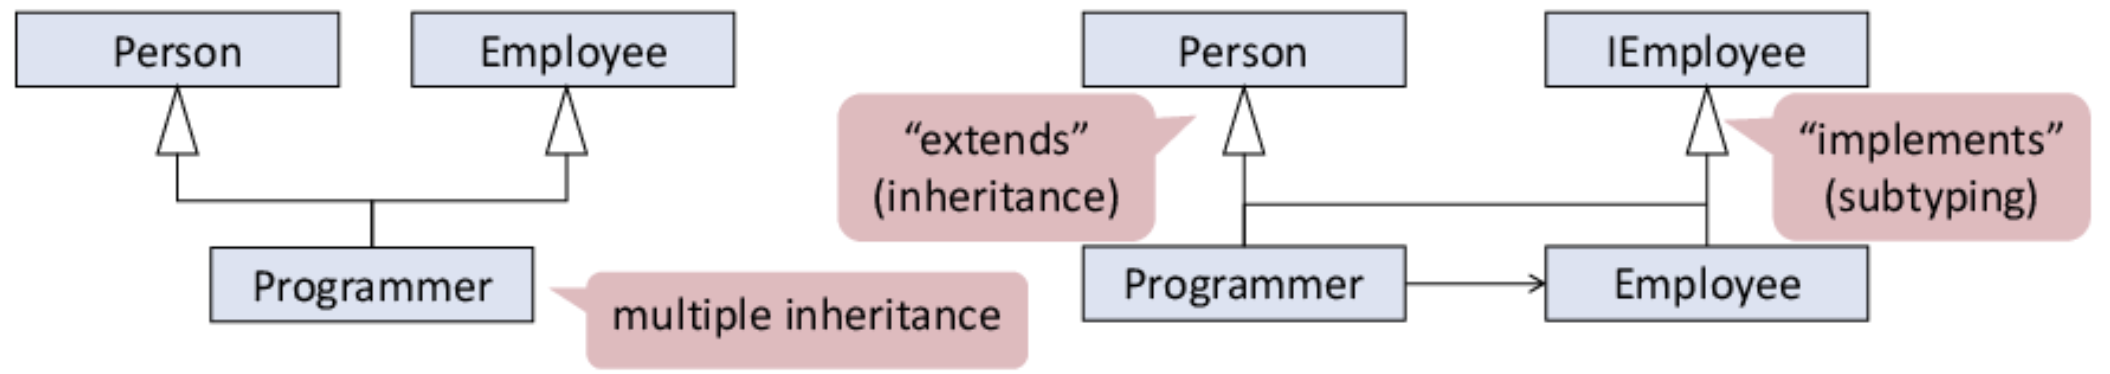
\includegraphics[width=\columnwidth]{assets/inheritance}
\end{center}

Using class names in declarations of methods, fields, and local variables couples the client to the used class. To avoid this, one can replace class names by supertypes (interfaces). Using the most general supertype that offers all required operations. \\

Lastly, allocations couples the client to the instantiated class. We fix this by using dedicated classes called abstract factories to handle allocation. 

\begin{center}
	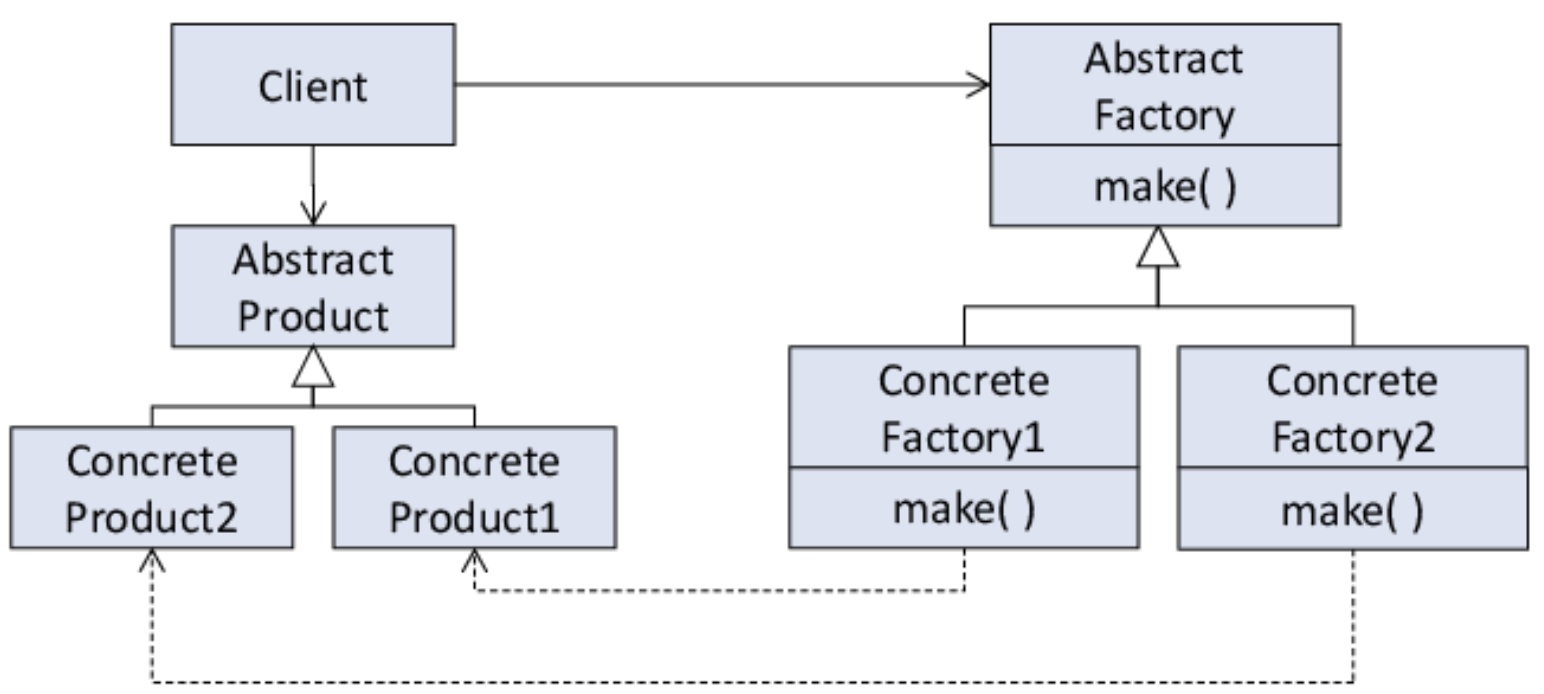
\includegraphics[width=0.7\columnwidth]{assets/factory}
\end{center}


\subsection{Adaption}

Changes often erode the structure of the system. Modules can be prepared for change by allowing clients to influence their behavior. This is done by making the module parametric in:
\begin{itemize}
	\item The value they manipulate
	\item The data structures they operate on
	\item The types they operate on
	\item The algorithms they apply
\end{itemize}

In object-oriented programs, behaviors can be specialized via overriding and dynamic method binding. Dynamic method binding is a case distinction on the dynamic type of the receiver object.